\chapter{Configurazione}
\label{Configurazione}
\thispagestyle{empty}

\section{Primo avvio}
Una volta eseguito Docker Compose, il sistema risulta avviato, funzionante e raggiungibile sulla porta 80, dall'host all'indirizzo \verb|localhost|, oppure da una macchina collegata alla rete locale tramite \verb|hostname|. Per quanto riguarda l'installazione fatta in ateneo, la macchine è raggiungibile all'indirizzo \verb|sharelatex.ing.unimore.it|, che verrà preso come esempio per i passi futuri.

Per prima cosa è necessario registrare l'amministratore del sistema all'indirizzo\\\verb|sharelatex.ing.unimore.it/launchpad|. Una volta inseriti indirizzo e-mail e password dell'amministratore, verrà richiesto il primo login. Inserite le credenziali dell'amministratore, verrà mostrata il launchpad, il quale mostra lo stato dell'editor e delle websocket e dal quale è possibile inviare un'email di test a un indirizzo a scelta\footnote{Per usufruire di questa funzionalità è necessario configurare il servizio mail con \href{SMTP}{SMTP}.}
\begin{figure}[h]
    \begin{subfigure}{0.5\textwidth}
        \centering
        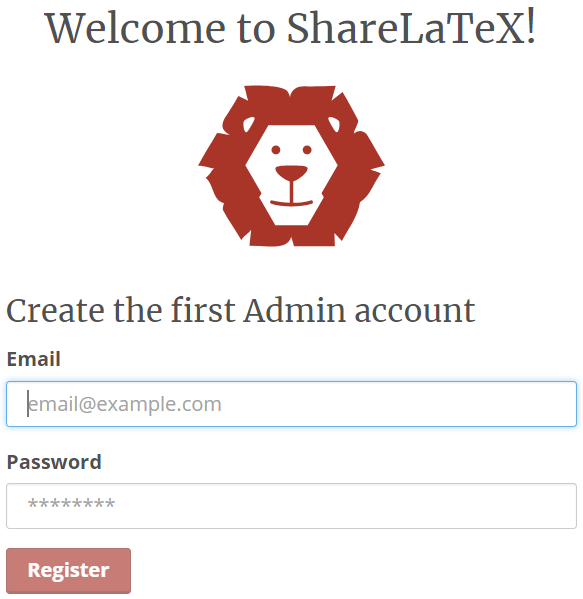
\includegraphics[height=7cm]{immagini/launchpad_1.png}
        \caption{Launchpad}
        \label{fig:sharelatex_launchpad_1}
    \end{subfigure}
    \begin{subfigure}{0.5\textwidth}
        \centering
        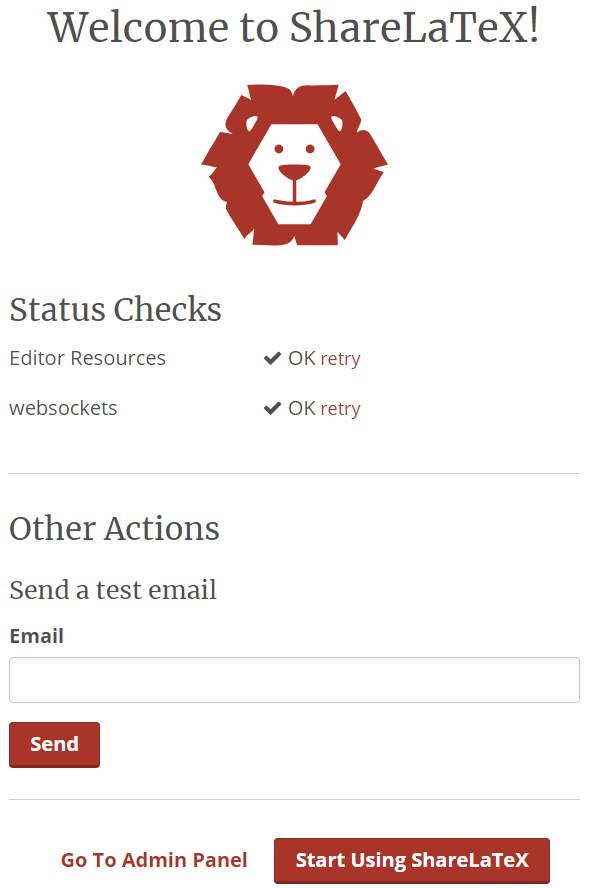
\includegraphics[height=7cm]{immagini/launchpad_2.png}
        \caption{Schermata di controllo}
        \label{fig:sharelatex_launchpad_2}
    \end{subfigure}
    \caption{Creazione utente amministratore}
    \label{fig:sharelatex_launchpad}
\end{figure}


\section{Interfaccia}
\verb|docker-compose.yml| permette di impostare variabili d'ambiente all'interno dei container. ShareLaTeX è altamente configurabile sotto questo aspetto. Si elencano le variabili d'ambiente utilizzate per l'installazione in ateneo.
\begin{itemize}
    \item \verb|SHARELATEX_APP_NAME|: nome dell'applicazione, che sarà mostrato nella barra di navigazione del browser.
    \item \verb|SHARELATEX_NAV_TITLE|: nome dell'applicazione, che sarà mostrato in alto a sinistra nell'homepage del profilo utente.
    \item \verb|SHARELATEX_HEADER_IMAGE|: URL di un'immagine, che sarà mostrata in alto a sinistra. Nel caso in cui \verb|SHARELATEX_NAV_TITLE| fosse impostato, allora\\\verb|SHARELATEX_HEADER_IMAGE| avrà la priorità.
    \item \verb|SHARELATEX_SITE_URL|: indirizzo della macchina host del servizio.
    \item \verb|SHARELATEX_ADMIN_EMAIL|: indirizzo e-mail dell'amministratore di sistema, che sarà mostrata in fase di registrazione utente.
    \item \verb|SHARELATEX_LEFT_FOOTER|: array JSON in cui si può aggiungere testo HTML che verrà mostrato in basso a sinistra nell'homepage.
    \item \verb|SHARELATEX_RIGHT_FOOTER|: array JSON in cui si può aggiungere testo HTML che verrà mostrato in basso a destra nell'homepage.
    \item \verb|SHARELATEX_SITE_LANGUAGE|: lingua dell'applicazione. Di default la lingua impostata è inglese, ma sono disponibili anche:
        \begin{multicols}{3}
            \begin{itemize}
                \item es = spagnolo
                \item pt = portoghese
                \item de = tedesco
                \item fr = francese
                \item cs = ceco
                \item nl = olandese
                \item sv = svedese
                \item it = italiano
                \item tr = turco
                \item cn = cinese
                \item no = norvegese
                \item da = danese
                \item ru = russo
                \item ko = coreano
                \item ja = giapponese
            \end{itemize}
        \end{multicols}
\end{itemize}

\section{SMTP}
\label{SMTP}
L'amministratore può registrare utenti normali all'applicazione aggiungendo la loro email nella pagina "Manage Users". La piattaforma genera un link per impostare la password del nuovo account. Questo link deve essere in qualche modo consegnato al nuovo utente. Se il servizio email è configurato, allora questa fase sarà automatica. I parametri sono passati mediante variabili d'ambiente. Si raccomanda impostare \verb|SHARELATEX_SITE_URL| per generare link di iscrizione funzionanti. Si elencano le variabili d'ambiente utilizzate per l'installazione in ateneo.
\begin{itemize}
    \item \verb|SHARELATEX_EMAIL_FROM_ADDRESS|: indirizzo del mittente del messaggio.
    \item \verb|SHARELATEX_EMAIL_SMTP_HOST|: host del servizio SMTP.
    \item \verb|SHARELATEX_EMAIL_SMTP_PORT|: porta SMTP da utilizzare.
    \item \verb|SHARELATEX_EMAIL_SMTP_SECURE|: valore booleano che, se vero, attiva SMTPS.
    \item \verb|SHARELATEX_EMAIL_SMTP_USER|: nome utente da autenticare.
    \item \verb|SHARELATEX_EMAIL_STMP_PASS|: password dell'utente da autenticare.
    \item \verb|SHARELATEX_EMAIL_STMP_TLS_REJECT_UNAUTH|: valore booleano che, se vero, rifiuta connessioni TLS (Transport Layer Security) non autorizzate.
    \item \verb|SHARELATEX_EMAIL_STMP_IGNORE_TLS|: valore booleano che, se vero, disattiva il supporto STARTTLS.
    \item \verb|SHARELATEX_CUSTOM_EMAIL_FOOTER|: testo HTML con cui si può personalizzare il footer delle email.
\end{itemize}

\section{TeX Live}
L'installazione completa dei pacchetti di TeX Live è essenziale per potere utilizzare qualsiasi pacchetto all'interno dei propri documenti. La totalità dei pacchetti occupa molta memoria sul disco (circa 7 GB), pertanto l'immagine di ShareLaTeX in Docker Hub presenta solo un'installazione parziale di TeX Live. La procedura di installazione richiederà inoltre molto tempo (circa 2 ore). La procedura risulta però ostacolata da un conflitto fra l'ultima versione disponibile di TeX Live (versione 2018) e quella installata sull'immagine \verb|sharelatex/sharelatex:v1.2.2| (versione 2017). Per risolvere qualche problema si è seguita la guida di aggiornamento fornita da TeX Live all'indirizzo \url{https://www.tug.org/texlive/upgrade.html}.

Si noti che il ripristino/ricreazione di un qualunque container eliminerà tutte le modifiche ad esso apportate. Ciò significa che un eventuale riavvio del container ShareLaTeX dopo l'installazione completa di TeX Live ripristinerebbe lo stato dell'installazione iniziale. Questo può succedere, ad esempio, a seguito di modifiche al file \verb|docker-compose.yml| e all'esecuzione di \verb|sudo docker-compose up -d|. Pertanto è opportuno montare un volume esterno in corrispondenza della directory /usr/local/texlive/2018 per rendere persistenti i file dell'aggiornamento.

\subsection{Fasi preliminari}
Modificare la variabile d'ambiente \verb|PATH|. Il modo più efficace e persistente consiste nell'aggiunta di \verb|PATH| fra le variabili d'ambiente di ShareLaTeX in \verb|docker-compose.yml|.
\begin{lstlisting}
environment:
    PATH: /usr/local/sbin:/usr/local/bin:/usr/sbin:/usr/bin:/sbin:/bin:/usr/local/texlive/2018/bin/x86_64-linux
\end{lstlisting}
Si noti che il ripristino/ricreazione di un qualunque container eliminerà tutte le modifiche ad esso apportate. Ciò significa che un eventuale riavvio del container ShareLaTeX dopo l'installazione completa di TeX Live ripristinerebbe lo stato dell'installazione iniziale. Questo può succedere, ad esempio, a seguito di modifiche al file \verb|docker-compose.yml| e all'esecuzione di \verb|sudo docker-compose up -d|. Pertanto è opportuno montare un volume esterno in corrispondenza della directory /usr/local/texlive/2018 per rendere persistenti i file dell'aggiornamento.
\begin{lstlisting}
volumes:
    - ~/sharelatex_texlive:/usr/local/texlive/2018
\end{lstlisting}
Salvare le modifiche e riavviare i container.
\begin{lstlisting}
sudo docker-compose up -d
\end{lstlisting}

\subsection{Aggiornamento}
È necessario avviare una bash all'interno del container ShareLaTeX. Docker permette di avviare comandi all'interno dei container mediante il comando \verb|exec|. Le opzioni \verb|-t| e \verb|-i| servono rispettivamente per creare una pseudo-TTY e per renderla interattiva con standard input.
\begin{lstlisting}
sudo docker exec -ti sharelatex bash
\end{lstlisting}
Una volta all'interno del container, visitare il percorso \verb|/usr/local/texlive| e copiare il contenuto della diretory \verb|2017| in \verb|2018| (generata dopo aver montato il volume e riavviato il container). Entrare succesivamente nella directory \verb|2018|.
\begin{lstlisting}
cd /usr/local/texlive
cp -a 2017/* 2018
cd 2018
\end{lstlisting}
Scaricare ed eseguire lo script d'aggiornamento \verb|update-tlmgr-latest.sh|.
\begin{lstlisting}
wget http://ctan.mirror.garr.it/mirrors/CTAN/systems/texlive/tlnet/update-tlmgr-latest.sh
sh update-tlmgr-latest.sh -- --upgrade
tlmgr update --self --all
\end{lstlisting}
Ripristinare la cache lualatex/fontspec (non essenziale).
\begin{lstlisting}
luaotfload-tool -fu
\end{lstlisting}
Infine uscire dal container con \verb|exit|.

\subsection{Installazione}
L'installazione completa di TeX Live sarà avviata tramite il comando \verb|exec| dall'esterno. L'operazione richiederà molto tempo.
\begin{lstlisting}
sudo docker exec sharelatex tlmgr install scheme-full
\end{lstlisting}
Attendere fino al termine dell'installazione. Eventuali interruzioni non comprometteranno l'installazione, che riprenderà da dove era stata interrotta.